Os Uses Cases são uma forma sistemática de capturar requisitos funcionais, fornecendo assim uma notação diagramática que permite modelar o contexto geral do sistema. Isto é, este diagrama representa os atores do Sistema (quem utiliza o Sistema), os use cases (o que se pode fazer no Sistema) e as associações entre os atores e os use cases. As entidades que consideramos serem as principais no sistema, isto é, as entidades que efetivamente vão interagir com ele são as seguintes: User e Admin. 

O primeiro ator que identificamos foi o Administrador, que é responsável pela gestão das contas, sendo esta gestão apenas representada por um use case: Eliminar Conta. Este também é responsável por Gerir Rotas. Para isto tem que se autenticar.

O ator que se segue é o Utilizador, e este tem acesso a tudo o que a aplicação fornece, e precisa de fazer login para se autenticar. 

Inicialmente consideramos o seguinte diagrama Use Cases:

\begin{figure}[H]
\centering
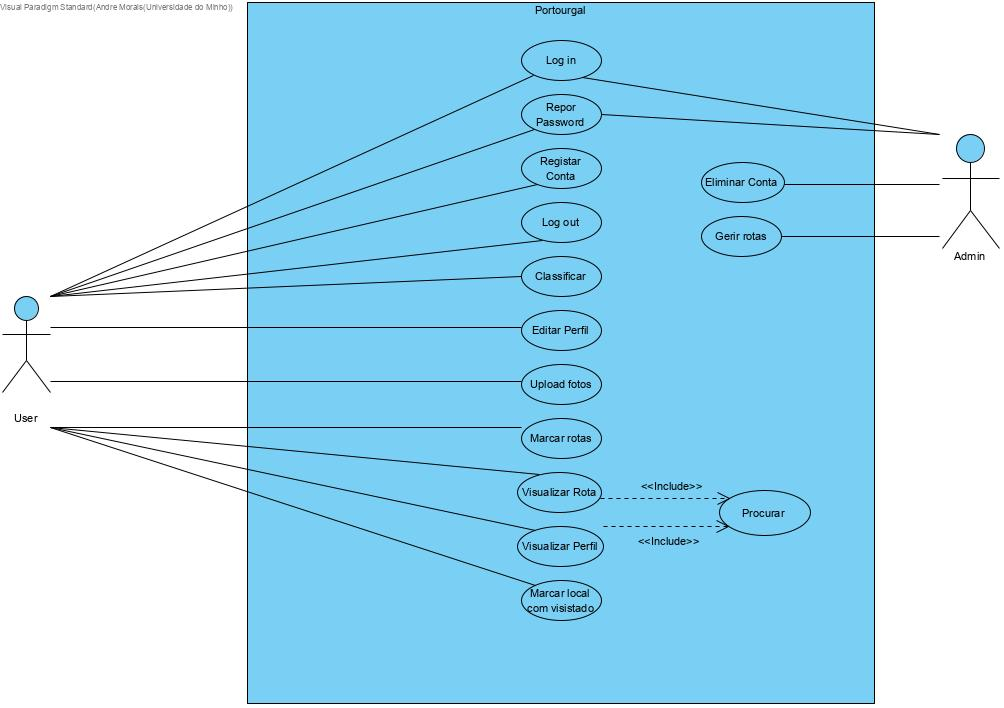
\includegraphics[width=0.9\linewidth]{images/usecases.jpg}
\caption{Diagrama de Use Cases inicial}
\label{fig:uc}
\end{figure}


\newpage

Depois de uma nova e mais profunda análise aos requisitos funcionais do sistema e aos Mockups desenvolvidos, decidimos que alguns Use Cases não iriam ser representados, portanto fomos removendo esses Use Cases do nosso diagrama. Removemos os use cases relativos à Search Bar, pois não seria necessário dado a nossa implementação do Front End da aplicação, isto é, a nível de apresentação da aplicação não iria ser necessário esta funcionalidade. O use case Upload de fotos poderia quebrar regras de segurança da aplicação, e teríamos que implementar um sistema de verificação de fotos, portanto decidimos, após uma conversa com o docente da U.C, retirar este use case. 

\begin{figure}[H]
\centering
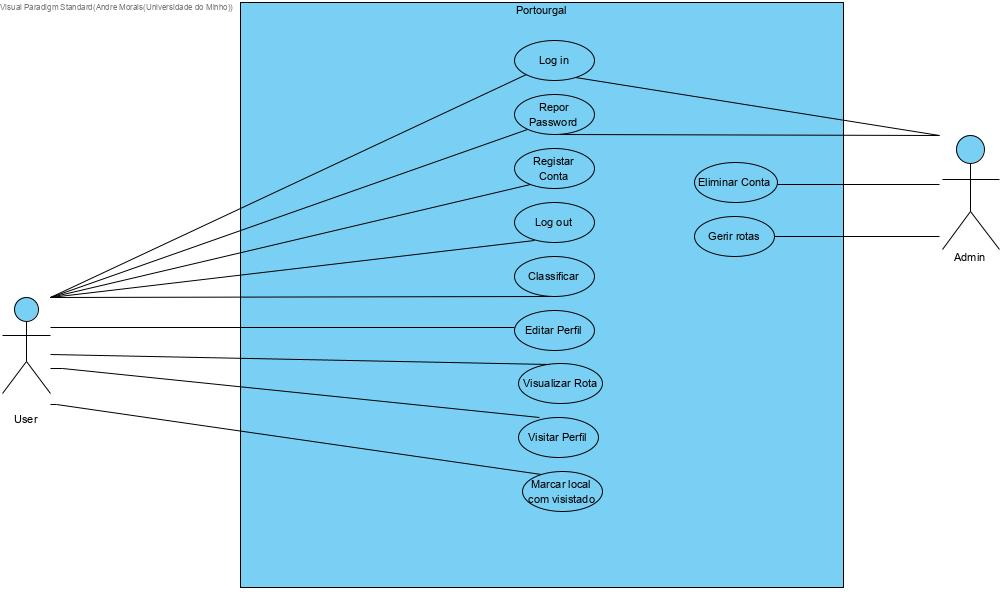
\includegraphics[width=0.9\linewidth]{images/usecases2.jpg}
\caption{Diagrama de Use Cases Final}
\label{fig:uc2}
\end{figure}
